%!TEX TS-program = pdflatex
%!TEX TS-options = -shell-escape
\newcommand{\setfontsize}{11pt}
\documentclass[%
	paper=a4,
	fontsize=\setfontsize,
	ngerman
	]{scrartcl}

% Basics für Codierung und Sprache
% ===========================================================
	\usepackage{scrtime}
	\usepackage{etex}
	\usepackage{shellesc}
	\usepackage[final]{graphicx}
	\usepackage[utf8]{inputenc}
	\usepackage{babel}
	\usepackage[german=quotes]{csquotes}
% ===========================================================

% Fonts und Typographie
% ===========================================================
	\usepackage{sourcecodepro}
	\usepackage[default]{sourcesanspro}
	\usepackage{nimbusmononarrow}
	
	\usepackage[babel=true,final,tracking=smallcaps]{microtype}
	\DisableLigatures{encoding = T1, family = tt* } % keine Ligaturen für Monospace-Fonts
	\usepackage{ellipsis}
% ===========================================================

% Farben
% ===========================================================
	\usepackage[usenames,x11names,final]{xcolor}
	\definecolor{fbblau}{HTML}{3078AB}
	\definecolor{mediumgray}{gray}{.65}
	\definecolor{blackberry}{rgb}{0.53, 0.0, 0.25}
% ===========================================================

% Mathe-Pakete und -Einstellungen
% ===========================================================
	\usepackage{mathtools}
	\usepackage{amssymb}
	\usepackage[bigdelims]{newtxmath}		% moderne Mathe-Font
	\allowdisplaybreaks						% seitenübergreifende Rechnungen
	\input{../MathCmds.tex}
	\usepackage{bm}
	\usepackage{wasysym}
% ===========================================================

% TikZ
% ===========================================================
	\usepackage{tikz}
	\usepackage{tikz-cd}					% kommutative Diagramme
	\usetikzlibrary{arrows.meta}			% mehr Pfeile!
	\usetikzlibrary{shadows}
	\usetikzlibrary{calc}
	\tikzset{>=Latex}						% Standard-Pfeilspitze
% ===========================================================

% Seitenlayout, Kopf-/Fußzeile
% ===========================================================
	\usepackage{scrpage2}
	\pagestyle{scrheadings}
	\usepackage[top=3cm, bottom=3cm, left=2.5cm, right=2cm]{geometry}
	\clearscrheadfoot 
	\setheadsepline{0.4pt} 					% Linie in Kopfzeile
	\setfootsepline{0.4pt}
	\automark[section]{section}				% Abschnittstitel in Kopfzeile
	\setkomafont{pagehead}{\bfseries}
	\setkomafont{pagefoot}{\normalfont\footnotesize}
	\cfoot{\thepage}
	\raggedbottom
	\usepackage{setspace}					
	\onehalfspacing							% Zeilenabstand 1.5-fach
	\setlength{\parindent}{0pt}
	\setlength{\parskip}{0.5\baselineskip}
	\usepackage[all]{nowidow}
% ===========================================================

% Hyperref
% ===========================================================
	\usepackage[%
		hidelinks,
		pdfpagelabels,
		bookmarksopen=true,
		bookmarksnumbered=true,
		linkcolor=black,
		urlcolor=SkyBlue2,
		plainpages=false,
		pagebackref,
		citecolor=black,
		hypertexnames=true,
		pdfauthor={Phil Steinhorst},
		pdfborderstyle={/S/U},
		linkbordercolor=SkyBlue2,
		colorlinks=false,
		backref=false]{hyperref}
	\hypersetup{final}
% ===========================================================

% Listen und Tabellen
% ===========================================================
	\usepackage{multicol}
	\usepackage[shortlabels]{enumitem}
	\setlist{itemsep=0pt}
	\setlist[enumerate]{font=\sffamily\bfseries}
	\setlist[itemize]{label=$\triangleright$}
	\usepackage{tabularx}
% ===========================================================

% Zu Testzwecken
% ===========================================================
	\usepackage{lipsum}
% ===========================================================

% Rechnerstrukturenquatsch
% ===========================================================
	\usepackage{karnaughmap}
% ===========================================================

% ntheorem
% ===========================================================
	\usepackage[amsmath]{ntheorem}
	
	\theoremstyle{default}
	\theoremseparator{.}
	\theorembodyfont{\normalfont}
	\theorempreskip{2em}
	\theorempostskip{2em}
	\newtheorem{aufg}{Aufgabe}

% minted
% ===========================================================
\usepackage{minted}
\setminted{%
	style=bw,
	fontsize=\normalsize,
	breaklines,
	breakanywhere=false,
	breakbytoken=false,
	breakbytokenanywhere=false,
	breakafter={.,},
	autogobble,
	numbersep=3mm,
	tabsize=4,
	frame=lines
}
\setmintedinline{%
	style=bw,
	fontsize=\normalsize,
	numbers=none,
	numbersep=12pt,
	tabsize=4,
	%bgcolor=gray!15,
}

\usepackage[tikz]{mdframed}
\newcommand{\code}[1]{\texttt{#1}}
\lohead{C++-Übungsaufgaben (3)}
\rohead{04.02.2019}
\rofoot{\jobname.tex}
\lofoot{}
\begin{document}

In dieser Aufgabe soll ein Datentyp \code{DVD} modelliert werden, um auf DVDs gespeicherte Spielfilme darstellen zu können. Gegeben ist dazu folgendes UML-Diagramm:

\begin{center}
	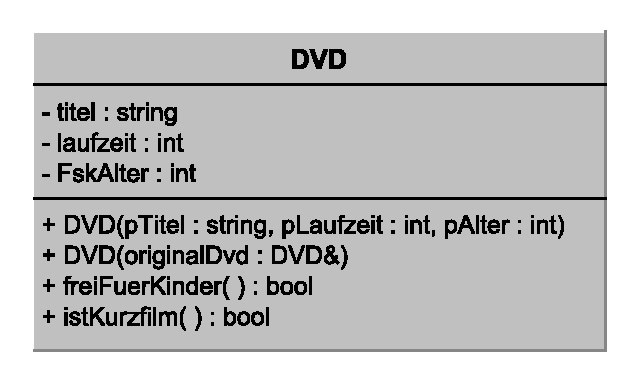
\includegraphics[keepaspectratio,scale=0.7]{dvd-uml.pdf}
\end{center}

\begin{enumerate}
	\item Erstellen Sie zu obigem Klassendiagramm eine Klassendefinition in C++ in einer separaten Schnittstellendatei \code{DVD.h}.
	Achten Sie darauf, dass ein mehrfaches Einbinden dieser Datei verhindert wird.
	\item Implementieren Sie die folgenden Methoden in einer C++-Datei \code{DVD.cpp}:
	\begin{enumerate}[(a)]
		\item Implementieren Sie den ersten Konstruktor. Dieser erhält als Parameter den Titel des Spielfilms, seine Laufzeit in Minuten und die Altersbeschränkung in Jahren, ab der der Film für Kinder und Jugendliche freigegeben ist.
		Verwenden Sie eine Initialisierungsliste, wenn möglich.
		\item Implementieren Sie den Kopierkonstruktor. Verwenden Sie eine Initialisierungsliste, wenn möglich.
		\item Implementieren Sie die Methoden \code{freiFuerKinder} und \code{istKurzfilm}. \code{freiFuerKinder} soll \code{true} zurückliefern, wenn die Altersbeschränkung maximal bei 6 Jahren liegt. \code{istKurzfilm} soll \code{true} zurückgeben, wenn die Spielzeit des Films maximal bei 40 Minuten liegt.
		\item Erstellen Sie Getter- und Setter-Methoden für alle drei Attribute.
	\end{enumerate}
	\item Ergänzen Sie alle Parameter und Methoden um das Schlüsselwort \code{const}, wo dies sinnvoll erscheint.
	\item Manchmal sollen zwei Spielfilme, die bereits auf DVD erschienen sind, gemeinsam auf einer neuen DVD veröffentlicht werden.
	Dies soll mithilfe des Operators \code{+} realisiert werden.
	Überladen Sie den Operator \code{+}, um zwei \code{DVD}-Objekte addieren zu können. Die Summe zweier \code{DVD}-Objekte ist ein neues \code{DVD}-Objekt mit folgenden Eigenschaften:
	\begin{itemize}
		\item Die Laufzeit der neuen DVD ist die Summe der Laufzeiten der beiden ursprünglichen DVDs.
		\item Die Altersbeschränkung ist das Maximum der Altersbeschränkungen der beiden ursprünglichen DVDs.
		\item Besitzt \code{dvd1} den Titel \enquote{Film 1} und \code{dvd2} den Titel \enquote{Film 2}, so besitzt \code{dvd1 + dvd2} den Titel \enquote{Film 1 und Film 2}.
	\end{itemize} 
	\item Erzeugen Sie in einer \code{main}-Methode zwei beliebige \code{DVD}-Objekte und addieren Sie sie. Geben Sie anschließend Titel, Laufzeit und Altersbeschränkung der addierten \code{DVD}-Objekte aus.
\end{enumerate}
\end{document}